\chapter{Giới thiệu đề tài}

\section{Giới thiệu về IoT}
Internet vạn vật (Internet of Things - IoT) hay mạng lưới vật kết nối, trong đó, các thiết bị, phương tiện, nhà cửa, ... được nhúng các thiết bị điện tử, phần mềm, cảm biến cùng khả năng kết nối tới mạng máy tính giúp cho các thiết bị này có thể thu thập và gửi dữ liệu. Hệ thống IoT cho phép vật được cảm nhận hoặc được điều khiển từ xa thông qua hạ tầng mạng hiện hữu, tạo cơ hội cho thế giới thực được tích hợp trực tiếp hơn vào hệ thống điện toán, hệ quả là hiệu năng, độ tin cậy và lợi ích kinh tế được tăng cường bên cạnh việc giảm thiểu sự can dự của con người. Mục đích của Internet vạn vật là tạo ra các liên kết Máy-Máy (Machine-to-Machine), được xem như là thông minh. Các thiết bị thu thập dữ liệu hữu ích rồi sau đó tự động truyền dữ liệu sang các thiết bị khác. Các ví dụ về IoT có thể kể đến như tự động bật tắt đèn, hệ thống thông gió, hệ thống điều hòa nhiệt độ, ... 

\subsection{Lịch sử của internet of things}
Năm 1999, Kevin Ashton, đồng sáng lập của trung tâm Auto-ID tại MIT, lần đầu tiên đề cập tới IoT trong bài trình bày của mình tại Procter \& Gamble (P\&G). Với mong muốn thu hút sự chú ý của các nhà quản lý của P\&G với công nghệ RFID (radio frequency ID), Ashton gọi bài trình bày của ông là "Internet of Things" để phù hợp với xu hướng đang nổi lúc bấy giờ là Internet. 

Đến  nay, IoT khẳng định được bước tiến của mình nhờ sự hội tụ của nhiều công nghệ, bao gồm truyền tải vô tuyến hiện diện dầy đặc, phân tích dữ liệu thời gian thực, học máy, cảm biến hàng hóa, và hệ thống nhúng. Điều này có nghĩa là tất cả các dạng thức của hệ thống nhúng cổ điển, như mạng cảm biến không dây, hệ thống điều khiển, tự động hóa (bao gồm nhà thông minh và tự động hóa công trình), vân vân đều đóng góp vào việc vận hành Internet Vạn Vật (IoT). 

Mặc dù Ashton là người đầu tiên đề cập tới cụm từ "Internet of Things", ý tưởng về kết nối các thiết bị đã xuất hiện từ khoảng những năm 1970, dưới cái tên Internet nhúng (embedded internet) và tính toán rộng khắp (pervasive computing). Thiết bị được kết nối internet đầu tiên trên thế giới là một máy bán Coca-Cola tại đại học Carnegie Mellon từ đầu những năm 1980, có khả năng báo cáo kiểm kho và báo cáo độ lạnh của những chai nước mới bỏ vào máy. 
Bản mô tả sơ khai năm 1991 về điện toán phổ quát (ubiquitous computing) của Mark Weiser, "Máy tính thế kỷ XXI", cũng như những báo cáo về tầm nhìn đương đại của IoT từ các viện khoa học UbiComp và PerCom. Năm 1994 Reza Raji mô tả khái niệm này trên tờ IEEE Spectrum là "chuyển các gói dữ liệu nhỏ sang tập hợp các nút mạng lớn, để tích hợp và tự động hóa mọi thứ từ các thiết bị gia dụng với cả một nhà máy sản xuất". Giữa năm 1993 và 1996 một số công ty đề xuất giải pháp như at Work của Microsoft hay NEST của Novell.  Tuy nhiên, chỉ đến năm 1999, lĩnh vực IoT mới bắt đầu có sự chuyển biến. Bill Joy mường tượng tới phương thức truyền tải thiết bị-tới-thiết bị (D2D) ở một phần trong bộ khung "Six Webs" của ông, được ông diễn thuyết tại Diễn đàn Kinh tế Thế giới ở Davos năm 1999. Khái niệm Internet Vạn Vật trở nên phổ biến trong năm 1999 nhờ Trung tâm Auto-ID ở Viện Công nghệ Massachusetts và các xuất bản phẩm phân tích thị trường có liên quan. Radio-frequency identification (RFID) được Kevin Ashton (một trong những sáng lập gia của trung tâm Auto-ID) cho rằng là điều kiện tiên quyết cho IoT. Ashton thích dùng cụm từ "Internet cho các vật" hơn. Nếu tất cả các đồ vật và con người trong cuộc sống thường ngày đều được mang định danh, máy tính có thể điều khiển và can thiệp vào. Bên cạnh việc sử dụng RFID, các nhãn của các vật cũng có thể thu được thông qua các công nghệ nhưu giao tiếp tầm gần (near field communication), barcode, QR code và digital watermarking.[41][42]

IoT được phát triển từ việc các máy tính giao tiếp với nhau -M2M (Machine-to-machine communication) thông qua một mạng máy tính mà không cần có sự can thiệp của con người. Trong M2M, các thiết bị được kết nối tới các đám mây tính toán (cloud computing), các đám mây sẽ thực hiện thu thập và quản lý dữ liệu. Đưa M2M đi xa hơn nữa, IoT là một mạng cảm biến với hàng tỷ thiết bị thông minh kết nối con người, các hệ thống và các ứng dụng để thu thập và chia sẻ dữ liệu. M2M chính là nền tảng cho sự kết nối để đạt được IoT.

IoT cũng là sự mở rộng tự nhiên của SCADA (supervisory control and data acquisition - giám sát điều khiển và thu thập dữ liệu), một loại chương trình ứng dụng để thực hiện điều khiển, thu thập dữ liệu thời gian thực từ xa để điều khiển thiết bị. Các hệ thống SCADA  bao gồm phần cứng và phần mềm. Thành phần phần cứng thu thập và chuyển dữ liệu đến máy tính có cài phần mềm SCADA, nơi dữ liệu sẽ được xử lý và hiển thị theo thời gian. Các thế hệ cuối của các hệ thống SCADA chính là thế hệ đầu tiên của hệ thống IoT. 
Khái niệm về hệ sinh thái IoT, lại không thực sự xuất hiện cho tới tận giữa năm 2010, khi chính phủ Trung Quốc nói rằng muốn IoT là mục tiêu chiến lược của mình trong kế hoạch năm năm.


\subsection{Lợi ích của internet of things}
Khi IoT được diễn ra phổ biến, sẽ dẫn tới quá trình tự động hóa đại trà trên nhiều lĩnh vực. Theo Garner, Inc.  (một công ty nghiên cứu và tư vấn về công nghệ), sẽ có khoảng 26 tỷ thiết bị IoT vào năm 2020. Theo một cuộc khảo sát và nghiên cứu gần đây được thực hiện bởi dự án Internet Pew Research, một phần lớn các chuyên gia công nghệ đã hưởng ứng tham gia sử dụng Internet of Things với 83% đồng ý quan điểm cho rằng Internet of Things sẽ có tác động rộng rãi và mang lại lợi ích đến năm 2025. 
Một số lợi ích của IoT với các doanh nghiệp có thể kể đến như sử dụng tài nguyên hiệu quả hơn, giảm công sức của con người đồng thời giảm chi phí và mang lại hoạt động hiệu quả hơn, nâng cao trải nghiệm người dùng, tiết kiệm thời gian và tiền bạc, ... Ngoài ra, đối với khách hàng, người sử dụng, những ngôi nhà thông minh có thể điều khiển từ xa, có các hệ thống điều khiển tự động giúp thuận tiện hơn cho người dùng; các thiết bị IoT có thể đeo được trên cơ thể con người giúp thu thập dữ liệu về con người, phân tích các dữ liệu đó và đưa ra các hỗ trợ cho con người ví dụ như trong các trường hợp y tế khẩn cấp, …

\subsection{Các công nghệ liên quan tới Internet of things}
\subsubsection{Phần cứng}

Thành phần phần cứng cơ bản nhất của một hệ thống IoT là các cảm biến. Một cách khái quát, một cảm biến là một thiết bị có khả năng phát hiện những thay đổi trong môi trường. Nếu hoạt động độc lập, một cảm biến sẽ là vô dụng, tuy nhiên, khi chúng ta dùng chúng trong một hệ thống điện tử, cảm biến đóng vai trò chính yếu. Một cảm biến  có thể đo đạc một hiện tượng vật lý (ví dụ như nhiệt độ, độ ẩm, áp suất, ...) và chuyển chúng thành các tín hiệu điện. Một cảm biến tốt cần phải có ba tính chất: Nhạy bén với các hiện tượng vật lý mà chúng đo đạc, không nhạy với các hiện tượng vật lý khác, và không làm thay đổi các giá trị đo trong quá trình đo đạc. Một số cảm biến phổ biến ngày nên có thể kể đến như cảm biến nhiệt độ, độ ẩm, ánh sáng, gia tốc, ... 

Để đọc các giá trị được tạo ra bởi các cảm biến, các cảm biến thường được kết nối tới một bảng mạch vi xử lý. Một số mạch vi xử lý như Arduino, Raspberry Pi, Intel Galileo, … trong đó Arduino được sử dụng phổ biến nhất bởi cả các chuyên gia lẫn những người mới bắt đầu. Arduino là một board mạch vi xử lý được sinh ra tại thị trấn Ivrea ở Ý, nhằm xây dựng các ứng dụng tương tác với nhau hoặc với môi trường được thuận lợi hơn. Phần cứng bao gồm một board mạch nguồn mở được thiết kế trên nền tảng vi xử lý AVR Atmel 8bit, hoặc ARM Atmel 32-bit. Những Model hiện tại được trang bị gồm 1 cổng giao tiếp USB, 6 chân đầu vào analog, 14 chân I/O kỹ thuật số tương thích với nhiều board mở rộng khác nhau. Được giới thiệu vào năm 2005, Những nhà thiết kế của Arduino cố gắng mang đến một phương thức dễ dàng, không tốn kém cho những người yêu thích, sinh viên và giới chuyên nghiệp để tạo ra những thiết bị có khả năng tương tác với môi trường thông qua các cảm biến và các cơ cấu chấp hành. Những ví dụ phổ biến cho những người yêu thích mới bắt đầu bao gồm các robot đơn giản, điều khiển nhiệt độ và phát hiện chuyển động. Đi cùng với nó là một môi trường phát triển tích hợp (IDE) chạy trên các máy tính cá nhân thông thường và cho phép người dùng viết các chương trình cho Arduino bằng ngôn ngữ C hoặc C++. Thông tin thiết kế phần cứng được cung cấp công khai để những ai muốn tự làm một mạch Arduino bằng tay có thể tự mình thực hiện được (mã nguồn mở). Người ta ước tính khoảng giữa năm 2011 có trên 300 ngàn mạch Arduino chính thức đã được sản xuất thương mại, và vào năm 2013 có khoảng 700 ngàn mạch chính thức đã được đưa tới tay người dùng. 
Sau khi đã đọc được dữ liệu từ các cảm biến, các mạch vi xử lý gửi dữ liệu tới các máy tính để lưu trữ, xử lý dữ liệu. Tuy nhiên, một số mạch vi xử lý không hỗ trợ các giao thức mạng như wifi, bluetooth nên cần các mạch bổ trợ như esp8266, module HC06, …

\begin{center}
	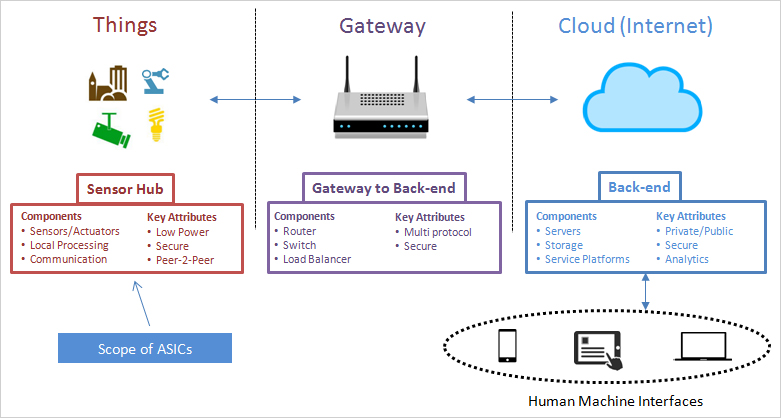
\includegraphics[scale=0.6]{image/internet-of-things1}
	Hình  : kiến trúc hệ thống IoT \\
	nguồn:http://www.open-silicon.com/wp-content/uploads/2015/05/internet-of-things1.jpg

\end{center}


\subsubsection{Các giao thức trong IoT}
Điều quan trọng trong Internet of Things là các thiết bị phải được đưa lên internet, tức là phải có một định danh duy nhất. Tuy nhiên, với giao thức IPv4, số lượng định danh có thể có là 232 tức hơn 4 tỷ định danh. Mặc dù có thể dùng các kỹ thuật để tăng số lượng IPv4 (ví dụ NAT, ...) tuy nhiên không thể giải quyết triệt để vấn đề này trong khi số lượng thiết bị IoT ngày càng tăng với tốc độ nhanh chóng và sẽ lên tới hàng chục tỷ thiết bị. Do đó giao thức IPv6 (có thể có 248 định danh) đang được tích cực triển khai để giải quyết vấn đề này. 

Một số giao thức truyền thông được sử dụng trong IoT là các giao thức truyền thông phổ biến như wifi, bluetooth, NFC, ... Tuy nhiên, cũng có các giao thức được sử dụng rộng rãi trong IoT nhưng ít được biết đến hơn như Zigbee, MQTT, AMQP, RFID, ... Zigbee là một giao thức mạng không dây được thiết kế chủ yếu cho môi trường công nghiệp với tần suất gửi dữ liệu nhỏ, phạm vi từ 10 tới 100m, ít tiêu thụ năng lượng, thường hoạt động ở tần số 2.4 GHz. MQTT (Message Queue Telemetry Transport) là một giao thức dựa trên cơ chế message - queue, sử dụng giao thức TCP để cung cấp cơ chế truyền tin đơn giản, tin cậy. Giao thức MQTT có ba thành phần chính: Subscriber, Publisher và Broker. Công việc của publisher là tạo ra dữ liệu và truyền dữ liệu cho subscriber với sự trợ giúp của broker; broker đảm bảo tính bảo mật, tin cậy dữ liệu bằng cách kiểm tra quyền truy nhật của subscriber và publisher. Giao thức MQTT là giao thức được ưu thích cho các thiết bị IoT do có khả năng cung cấp đủ chức năng về thông tin cho các thiết bị nhỏ, ít bộ nhớ và ít tiêu thụ dữ liệu, làm việc trên các mạng bị giới hạn về băng thông. Tương tự như MQTT, AMQP (Advanced Message Queuing Protocol) cũng là một giao thức dựa trên cơ chế message-queue nhưng phức tạp hơn MQTT và cung cấp các tính năng nâng cao hơn MQTT.

Mạng không dây thế hệ thứ năm 5G hứa hẹn có tốc độ lớn hơn nhiều so với hiện tại và có khả năng kết nối đồng thời nhiều hơn các thiết bị thông minh. Mạng nhanh hơn đồng nghĩa với việc dữ liệu từ các thiết bị thông minh sẽ được thu thập, phân tích và xử lý với cấp độ cao hơn. Đây sẽ là nguồn năng lượng sáng tạo cho các công ty tạo ra các thiết bị IoT và thúc đẩy nhu cầu của khách hàng cho các sản phẩm mới. 


\subsubsection{Các IoT platform}
IoT platform là một phần mềm giúp hỗ trợ quản lý các thiết bị, giúp đơn giản hóa việc giao tiếp, luồng dữ liệu, quản lý thiết bị và các chức năng của các ứng dụng. Nó đóng vai trò là lớp trung gian giữa tầng thiết bị và tầng ứng dụng. Công việc chủ yếu của nó bao gồm thu thập dữ liệu từ thiết bị thông qua các giao thức, mô hình mạng khác nhau, điều khiển và cấu hình các thiết bị. 

\begin{center}
	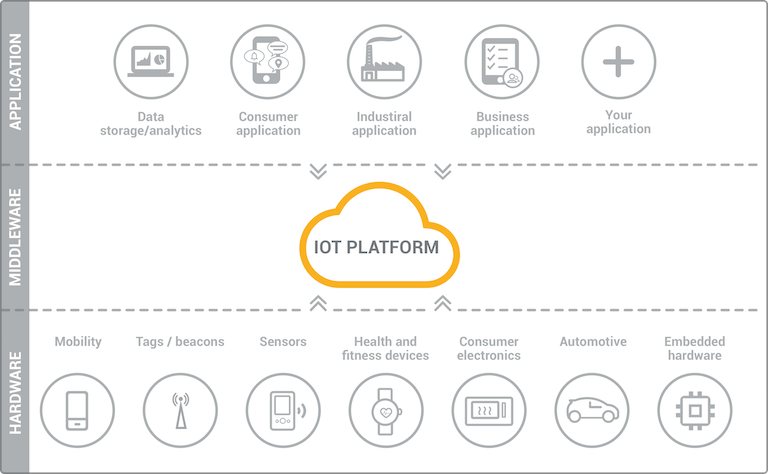
\includegraphics[scale=0.6]{image/IoTPlatform}
	Hình : IoT Platform \\
	nguồn: https://www.kaaproject.org/uploads/2016/12/WhatisIoTPlatform\_05-768x474.png
\end{center}

Theo thống kê của công ty nghiên cứu thị trường IoT-Analytics của Đức năm 2017 đã có khoảng 450 IoT Platform theo [2]. Một số IoT Platform đóng được dùng phổ biến như Google Cloud Platform, Saleforce IoT Cloud, IBM Wastson IoT, AWS IoT, ... Ngoài ra, các cộng đồng mã nguồn mở cũng có một số IoT Platform phổ biến như OpenHAB, HomeAssistant, ThingsBoard, …

\subsection{Bảo mật và an toàn trong IoT}
Vấn đề bảo mật trong IoT đã trở thành một chủ đề thu hút được nhiều sự chú ý sau một loạt các vụ tấn công nghiêm trọng có liên quan tới các thiết bị IoT được sử dụng để xâm nhập và tấn công các mạng máy tính lớn. Việc thực hiện các biện pháp bảo mật đóng vai trò hết sức quan trọng trong việc đảm bảo mạng các thiết bị IoT 
được kết nối tới nhau an toàn.

Có một số thách thức ngăn cản sự bảo mật của các thiết bị IoT và đảm bảo bảo mật cho toàn bộ môi trường IoT. Ý tưởng về việc kết nối các thiết bị và các vật thành một mạng vẫn còn tương đối mới, do đó vấn đề bảo mật không phải luôn được xem như là ưu tiên trong suốt quá trình thiết kế sản phẩm. Thêm vào đó, vì IoT là một thị trường mới, nhiều nhà thiết kế sản phẩm và các công ty quan tâm tới việc đưa sản phẩm của họ ra thị trường hơn việc xây dựng cơ chế bảo mật ngay từ đầu. Vấn đề chính được nêu ra với việc bảo mật trong IoT là việc sử dụng các mật khẩu mặc định, có thể dẫn tới sự xâm nhập an ninh trái phép và dù mật khẩu được đổi, chúng lại thường không đủ mạnh để ngăn chặn truy nhập trái phép. Một vấn đề phổ biến khác là các thiết bị IoT thường bị giới hạn về tài nguyên và không đủ năng lực tính toán cần thiết để cài đặt hệ thống bảo mật mạnh. Do đó, rất nhiều thiết bị không hoặc không thể cung cấp các tính năng bảo mật nâng cao. Ví dụ, một cảm biến nhiệt độ, độ ẩm không thể cài đặt cơ chế mã hóa hay các cơ chế bảo mật khác. Thêm vào đó, nhiều thiết bị IoT được đặt trong một cái máy và ở đó cho tới khi không sử dụng được nữa, chúng khó lòng được cập nhật các phiên bản bảo mật mới. Từ góc nhìn nhà sản xuất, xây dựng cơ chế bảo mật từ đầu vì có thể sẽ tốn kém, làm chậm quá trình phát triển.

Một số sự kiện về lỗ hổng, thâm nhập trái phép các thiết bị trong IoT đã được ghi nhận. Năm 2010, các nhà nghiên cứu đã phát hiện vi rút Stuxnet được sử dụng để gây thiệt hại tới các máy li tâm của Iran, các cuộc tấn công bắt đầu từ năm 2006 nhưng chủ yếu xảy ra vào năm 2009. Thường được xem là ví dụ đầu tiên của việc tấn công mạng IoT, Stuxnet nhắm vào hệ thống giám sát và thu thập dữ liệu (SCADA) với hệ thống điều khiển công nghiệp (ICS), sử dụng mã độc để đầu đọc các lệnh gửi từ bộ điều khiển logic (PLC). Các vụ tấn công vào hệ thống công nghiệp vẫn tiếp tục diễn ra, với các mã độc như CrasshOverride, Triton, VPNFilter, …
Tháng 12 năm 2013, một nhà nghiên cứu tại công ty bảo mật Proofpoint Inc. đã mô tả mạng IoT botnet đầu tiên. Theo đó, hơn 25\% của botnet được tạo ra từ các thiết bị IoT như smart TV, hệ thống giám sát trẻ và các đồ dùng trong nhà. Năm 2015, nhà nghiên cứu bảo mật Charlie Miller và Chris Valasek đã thực hiện hack vào một xe Jeep bằng mạng không dây, điều chỉnh máy phát radio trên xe, máy lạnh và dừng cảm biến gia tốc. Họ còn nói rằng, họ có thể tắt máy, phanh xe và tắt phanh. Miller và Valasek còn có thể thâm nhập vào mạng của chiếc xe thông qua hệ thống trong chiếc xe. 
Tháng 1 năm 2017, FDA cảnh báo hệ thống nhúng trong các thiết bị tim như máy điều hòa nhịp tim, máy khử rung tim và các thiết bị bất đồng bộ có thể bị tổn thương do các lỗ hổng bảo mật.

\subsection{Các dự đoán về IoT}
Một số dự đoán về tương lai của IoT đã được đưa ra. Theo IoT Analytics, năm 2016 có khoảng 4.7 tỷ thiết bị, và tới năm 2021 số lượng thiết bị sẽ đạt tới 21 tỷ thiết bị. Nhờ sự phát triển của IoT, ngày càng nhiều thiết bị, nhà cửa, thành phố sẽ trở nên thông minh hơn, trong đó các thành phố sẽ có khả năng tự động một số công việc, quản lý từ xa và thu thập dữ liệu thông qua các ki-ốt, camera giám sát, các trạm cho thuê xe, ... Khi dữ liệu trở nên nhiều hơn, trí thông minh nhân tạo AI sẽ đóng vai trò quan trọng hơn. Học máy, một lĩnh vực trong AI sẽ giúp máy tính có thể "học" để đưa ra các gợi ý mang tính cá nhân hóa cao hơn. Trong lĩnh vực bảo mật, tội phạm mạng vẫn sẽ tiếp tục sử dụng các thiết bị IoT để thực hiện các cuộc tấn công DDos. Bên cạnh đó, mối quan tâm về bảo mật và quyền riêng tư sẽ dành nhiều hơn cho tính pháp lý và các quy định về dữ liệu, đảm bảo quyền bảo mật thông tin cá nhân của người dân tốt hơn.


\section{Giới thiệu về truy vấn ngữ nghĩa}
\subsection{Ngôn ngữ truy vấn ngữ nghĩa}
Ngôn ngữ truy vấn ngữ nghĩa là ngôn ngữ truy vấn cho phép truy vấn và phân tích ngữ cảnh tự nhiên của câu truy vấn. Truy vấn ngữ nghĩa cho phép lấy ra các thông tin rõ ràng cũng như các thông tin ẩn về dữ liệu. Để xây dựng cơ chế truy vấn ngữ nghĩa, ta cần xây dựng mô hình mối quan hệ của các dữ liệu, một trong những cách để thực hiện là xây dựng ontology.

\subsection{Ontology}
\subsubsection{Khái niệm ontology}
Lịch sử của trí tuệ nhân tạo cho thấy rằng tri thức đóng vai trò hết sức quan trọng trong các hệ thống thông minh. Trong rất nhiều trường hợp, tri thức tốt có thể quan trọng hơn các giải thuật trong việc giải quyết một bài toán. Để có được một hệ thống thực sự thông minh, trí thức cần được thu thập, xử lý, tái sử dụng và được trao đổi. Ontology hỗ trợ tất cả các công việc này. Khái niệm ontology có thể được định nghĩa như sự cụ thể hóa một cách rõ ràng các khái niệm trong một miền lĩnh vực. Ontology thể hiện cấu trúc của miền lĩnh vực, bao gồm cả các mối quan hệ ràng buộc của các thành phần trong lĩnh vực đó. Các khái niệm trong một lĩnh vực thường không thay đổi hoặc rất ít thay đổi, và ontology là một bản mô tả các khái niệm trong lĩnh vực đó dựa trên ngôn ngữ mô hình hóa và các từ vựng cụ thể. Việc mô tả một cách hình thức ontology là yêu cầu bắt buộc để có thể xử lý và thực hiện các thao tác một các tự động trên ontology. Để xây dựng được ontology, ta cần xác định một cách hình thức các thành phần trong ontology như các thực thể của một khái niệm, các lớp (khái niệm), các thuộc tính của các khái niệm và mối quan hệ cũng như các ràng buộc, các luật, các tiên đề giữa các khái niệm. 

Các thực thể là một thành phần cơ bản của ontology. Các thực thể trong một ontology có thể là các đối tượng cụ thể ví dụ như một người cụ thể, một con vật cụ thể, một hành tinh cụ thể, ... 

Lớp hay khái niệm có thể được định nghĩa là một tập trừu tượng của các đối tượng. Các khái niệm có thể phân loại các thực thể của các đối tượng hoặc cũng có thể phân loại các khái niệm khác. Ví dụ, "động vật" là một khái niệm chỉ chung các cá thể động vật như chim, cá, hổ, báo, sư tử, con người, ... "Con người" lại có thể là một khái niệm chỉ tất cả những người sống trên Trái Đất. 

Các đối tượng trong một ontology có thể được mô tả bởi liên kết chúng tới các thành phần, các khía cạnh, ... của nó. Những thành phần, khía cạnh này được gọi là các thuộc tính tính. Mỗi thuộc tính cũng có thể là một lớp hay một thực thể. Ví dụ, "con người" có thể có thuộc tính "giới tính", "tên", "tuổi", ...
 
Mối quan hệ giữa các khái niệm trong một ontology xác định xem khái niệm này có liên quan tới khái niệm khác như thế nào. Ví dụ, khái niệm "con người" có mối quan hệ "là một loài" với khái niệm "động vật". Biểu diễn trở thành:
"con người" là một loài "động vật" 
Sức mạnh của ontology đến từ khả năng miêu tả các mối quan hệ giữa các khái niệm. Tập các mối quan hệ sẽ mô tả tính ngữ nghĩa của lĩnh vực. Một loại quan hệ rất quan trọng trong ontology là mối quan hệ: một khái niệm là khái niệm cha của một khái niệm khác. Ví dụ, "ô tô" là khái niệm cha của "ô tô bốn bánh". Ngược lại với mối quan hệ trên là mối quan hệ: một khái niệm là khái niệm con của một khái niệm khác. Ví dụ, "ô tô bốn bánh" là khái niệm con của "ô tô". Một mối quan hệ thường dùng khác là mối quan hệ: một khái niệm là một phần của một khái niệm khác. Ví dụ, "bánh xe", "cửa sổ" là một phần của "ô tô". 

Tập luật  là các mệnh đề dưới dạng điều kiện - kết quả (nếu-thì), dùng để mô tả phép suy dẫn logic từ một tập các mối quan hệ. Ví dụ, "nếu" "cá voi" là một loài "động vật"  và "động vật" là một loài "sinh vật" "thì" "cá voi" là một loài sinh vật.

Các tiên đề là các khẳng định mang tính logic. Ví dụ "memo" là một "con cá" và "mọi con cá" đều biết bơi nên "memo" biết bơi. 

\begin{center}
	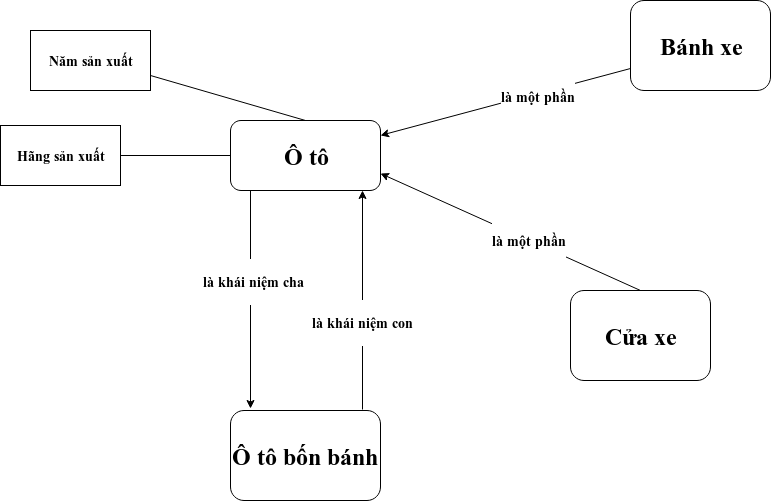
\includegraphics[scale=0.6]{image/otology_example}
\end{center}

Ontology không chỉ là bản mô tả có thể chia sẻ và tái sử dụng của một lĩnh vực mà còn có thể thêm các tri thức mới về lĩnh vực đó. 
Có một số cách khác có thể được sử dụng để mô tả một cách hình thức tri thức về một miền lĩnh vực như cơ sở dữ liệu quan hệ, sử dụng tập từ vựng của lĩnh vực, ... tuy nhiên, ontology nhấn mạnh mối quan hệ giữa các khái niệm và cho phép người sử dụng liên kết các khái niệm này với các khái niệm khác theo nhiều cách khác nhau. 

\subsubsection{Cách xây dựng một ontology}

Có nhiều phương pháp để xây dựng một ontology, tuy nhiên, nhìn chung, các phương pháp đều thực hiện hai bước cơ bản: xây dựng cấu trúc lớp phân cấp và định nghĩa các thuộc tính cho các lớp. Trong thực tế, để xây dựng một ontology mô tả một lĩnh vực là một công việc khó khăn, phụ thuộc rất nhiều vào công cụ sử dụng, tính chất, quy mô, sự thường xuyên biến đổi của lĩnh vực đó, cũng như các mối quan hệ phức tạp trong đó. Những khó khăn này đòi hỏi quá trình xây dựng ontology phải là một quá trình lặp đi lặp lại, mỗi lần lặp cải thiện, tinh chế và phát triển dần sản phẩm chứ không phải là một quy trình với các công đoạn tách rời nhau. Công việc xây dựng ontology cũng cần phải tính đến khả năng mở rộng lĩnh vực quan tâm trong tương lai, khả năng kế thừa các ontology đã có, cũng như có tính linh động để ontology có khả năng mô tả tốt nhất các mối quan hệ phức tạp trong thế giới thực. 
Một số nguyên tắc cơ bản trong xây dựng ontology:
Không có một cách duy nhất nào để mô hình hóa một lĩnh vực. Luôn có rất nhiều cách có thể thay thế cho nhau. Việc xác định cách tốt nhất thường phụ thuộc vào ứng dụng của mô hình và các mở rộng trong tương lai mà ta đoán trước sẽ có thể xảy ra.
Quá trình phát triển ontology là một quá trình lặp đi lặp lại
Các khái niệm trong ontology nên sát với các đối tượng (vật lý hoặc logic) trong lĩnh vực mà nó mô tả. Các khái niệm thường là những danh từ, các mối quan hệ thường là những động từ được dùng trong lĩnh vực.
Do đó, việc quyết định xem ontology dùng để làm gì và mức độ chi tiết hay tổng quát của ontology sẽ ảnh hưởng tới các quyết định trong khi xây dựng ontology. Trong rất nhiều các lựa chọn, chúng ta phải xác định lựa chọn nào sẽ phù hợp nhất với mục đích của ứng dụng, lựa chọn nào sẽ giúp ontology có khả năng mở rộng và có tính ổn định cao. Chúng ta cũng cần nhớ rằng một ontology là một bản mô tả một phần của thế giới và các khái niệm trong ontology phải phản ánh được phần thế giới đó. Sau khi ta đã tạo ra được một phiên bản đầu tiên của một ontology, ta có thể đánh giá, sửa đổi nó dựa trên ứng dụng sử dụng nó,  dựa trên ý kiến của các chuyên gia trong lĩnh vực,... Quá trình sửa đổi này sẽ tiếp tục cho tới hết vòng đời sử dụng của ontology.
Về cơ bản, việc xây dựng ontology cần thực hiện các bước sau:

Bước 1: Xác định lĩnh vực và phạm vi của ontology

Thông thường, các yêu cầu đối với một hệ thống Ontology là mô tả lĩnh vực quan tâm nhằm phục vụ cơ sở tri thức trong việc giải quyết những mục đích chuyên biệt. Công việc đặc tả để xác định, phân tích, nhận diện chính xác yêu cầu được thực hiện bằng cách trả lời những câu hỏi sau:
Ontology cần mô tả lĩnh vực nào?
Mục đích sử dụng ontology
Cơ sở tri thức trong Ontology sẽ giải quyết những câu hỏi gì?
Ai là người sẽ xây dựng, quản trị Ontology?
Nhìn chung, câu trả lời cho các câu hỏi dạng này có thể sẽ thường xuyên thay đổi trong suốt quá trình xây dựng một Ontology. Nhất là khi có sự thay đổi về mục đích hoặc cần bổ sung tính năng trong việc sử dụng cơ sở tri thức. Tuy nhiên, việc trả lời chính xác các câu hỏi trên tại mỗi bước lặp sẽ giúp giới hạn phạm vi của mô hình cần mô tả và dự trù các kỹ thuật sẽ sử dụng trong quá trình phát triển. Lấy ví dụ, nếu dự trù khả năng xảy ra sự khác biệt về ngôn ngữ giữa người phát triển và người sử dụng thì Ontology phải được bổ sung cơ chế ánh xạ (mapping) qua lại các thuật ngữ giữa các ngôn ngữ khác nhau. Hoặc giả sử Ontology cần xây dựng có chức năng xử lý ngôn ngữ tự nhiên, ứng dụng dịch tài liệu tự động thì cũng cần thiết phải có kỹ thuật xác định từ đồng nghĩa. Sau khi đã phát thảo phạm vi Ontology dựa trên việc trả lời những câu hỏi trên, người thiết kế sẽ trả lời các câu hỏi mang tính đánh giá, qua đó tiếp tục tinh chỉnh lại phạm vi của hệ thống cần xây dựng. Các câu hỏi dạng này thường dựa trên cơ sở tri thức của Ontology và được gọi là câu hỏi kiểm chứng khả năng (competency question):
Ontology đã có đủ thông tin để trả lời cho các câu hỏi được quan tâm trên cơ sở tri thức hay không?
Câu trả lời của cơ sở tri thức đã đáp ứng được mức độ, yêu cầu nào của người sử dụng?
Các ràng buộc và quan hệ phức tạp trong miền quan tâm đã được biểu diễn hợp lý chưa? 

Bước 2: Xem xét việc kế thừa các Ontology có sẵn:
Đây là một công đoạn thường hay sử dụng để giảm thiểu công sức xây dựng một Ontology. Bằng cách kế thừa các Ontology tương tự có sẵn, người xây dựng có thể thêm hoặc bớt các lớp, quan hệ giữa các lớp, thực thể để tinh chỉnh tùy theo mục đích của mình. Việc sử dụng lại các Ontology có sẵn cũng rất quan trọng khi cần sự tương tác giữa các ứng dụng khác nhau, các ứng dụng sẽ cần phải hiểu các lớp, thực thể, quan hệ của nhau để thuận tiện trong việc trao đổi hoặc thống nhất thông tin.
Vấn đề xây dựng một Ontology mới bằng cách kế thừa các hệ thống có sẵn liên quan đến một bài toán rất phức tạp là trộn (merging) các Ontology. Ví dụ trong trường hợp tên các khái niệm được định nghĩa trong các Ontology này có thể giống nhau trong khi chúng được dùng để mô tả các loại vật hoàn toàn khác nhau, và cũng có thể xảy ra trường hợp ngược lại, khi tên các khái niệm khác nhau nhưng cùng mô tả một sự vật, và một vấn đề nữa là làm thế nào để bổ sung các quan hệ, thuộc tính có sẵn vào một hệ thống mới. Tuy nhiên, hầu hết các Ontology sử dụng trong ngành khoa học máy tính nói chung và Web ngữ nghĩa nói riêng đều được xây dựng trên các hệ thống xây dựng và quản trị Ontology. Tên một số công cụ như: Sesame, Protégé, Ontolingua, Chimaera, OntoEdit, OidEd Hiện nay, đa số các phần mềm này đều hỗ trợ chức năng tự động trộn các Ontology cùng hoặc thậm chí khác định dạng với nhau. Mặc dù vậy, ở mức nào đó, người xây dựng cũng cần phải kiểm tra lại một cách thủ công, nhưng đây không phải là một công việc phức tạp. Hiện có rất nhiều Ontology được chia sẻ trên Web nổi tiếng như: UNSPSC (www.unspsc.org) do chương trình phát triển của Liên Hiệp Quốc hợp tác với tổ chức Dun \& Bradstreet nhằm cung cấp các thuật ngữ của các sản phẩm và dịch vụ thương mại. Các
Ontology trong lĩnh vực thương mại khác như: RosettaNet (www.rosettanet.org), DMOZ (www.dmoz.org), eClassOwl Open Biological, BioPax trong lĩnh vực sinh vật học, UMLS trong lĩnh vực mạng ngữ nghĩa, GO (Gene Ontology), WordNet (đại học Princeton).

Bước 3: Liệt kê các thuật ngữ quan trọng trong Ontology:
Đây là bước rất hữu ích, làm tiền đề cho hai bước tiếp theo là xây dựng cấu trúc lớp phân cấp và định nghĩa các thuộc tính cho lớp. Công đoạn này bắt đầu bằng việc liệt kê tất cả các thuật ngữ xuất hiện trong miền quan tâm (có thể đồng nghĩa hoặc chồng nhau)như tên khái niệm, quan hệ, thuộc tính. Thông thường, các thuật ngữ là danh từ sẽ trở thành các lớp, tính từ sẽ trở thành thuộc tính, còn động từ sẽ là quan hệ giữa các lớp. 

Bước 4: Xây dựng các lớp/khái niệm và cấu trúc lớp/khái niệm phân cấp:
Đây là một trong hai bước quan trọng nhất của công việc xây dựng một Ontology. Nhiệm vụ của bước này là định nghĩa các lớp từ một số thuật ngữ đã liệt kê trong bước trên, sau đó xây dựng cấu trúc lớp phân cấp theo quan hệ lớp cha-lớp con. Lớp ở vị trí càng cao sẽ có mức độ tổng quát càng cao. Vị trí đầu tiên thuộc về lớp gốc, tiếp theo là các lớp trung gian, và cuối cùng là lớp lá. Lớp lá là lớp không thể triển khai được nữa và chỉ được biểu hiện bằng các thực thể. Quan hệ giữa thực thể của lớp con với lớp cha là quan hệ "là một", nghĩa là một thực thể của lớp con cũng “là-một” thực thể của lớp cha. Có nhiều hướng tiếp cận khác nhau cho vấn đề
xây dựng cấu trúc lớp phân cấp. Có thể kể ra ba hướng như sau: 
Hướng xây dựng từ trên xuống (top-down): bắt đầu bằng các lớp có mức độ tổng quát cao nhất, sau đó triển khai dần đến lớp lá.
Hướng xây dựng từ dưới lên (bottom-up): ngược với hướng xây dựng cấu trúc lớp phân cấp từ trên xuống, hướng này bắt đầu bằng việc xác định các lớp được cho là cụ thể nhất, sau đó tổng quát hóa đến khi được lớp gốc.
Cách kết hợp (combination): cách này kết hợp cả hai hướng xây dựng trên. Đầu tiên chọn các lớp nổi bật nhất trong lĩnh vực quan tâm, sau đó tổng quát hóa và cụ thể hóa cho đến khi được cấu trúc mong muốn. 
Không có phương pháp nào trong ba phương pháp này là tốt nhất trong mọi trường hợp. Việc lựa chọn phương pháp nào phụ thuộc vào góc nhìn cá nhân của người xây dựng vào lĩnh vực. Nếu người xây dựng có một cái nhìn hệ thống từ trên xuống thì phương pháp xây dựng từ trên xuống sẽ phù hợp. Ngược lại, một người có cái nhìn từ dưới lên sẽ phù hợp với cách xây dựng từ dưới lên. Phương pháp kết hợp thường là cách dễ nhất cho những người xây dựng. 

Bước 5: Định nghĩa các thuộc tính và quan hệ cho lớp:
Bản thân các lớp nhận được ở bước trên chỉ mới là những thuật ngữ phân biệt với nhau bằng tên gọi. Về cơ bản, chúng chưa đủ để phục vụ cho việc biểu diễn tri thức. Muốn như vậy, các thuộc tính của lớp cần được định nghĩa. Thuộc tính của lớp là các thông tin bên trong của lớp, mô tả một khía cạnh nào đó của lớp và được dùng để phân biệt với các lớp khác. Thuộc tính được chia làm nhiều loại khác nhau:
Về mặt ý nghĩa, các thuộc tính có thể được chia làm hai loại: thuộc tính bên trong
(intrinsic property) và thuộc tính bên ngoài (extrinsic property). Thuộc tính bên trong mô tả các tính chất nội tại bên trong sự vật, ví dụ: chất, lượng, cấu tạo. Trong khi đó, thuộc tính bên ngoài mô tả phần biểu hiện của sự vật, ví dụ: màu sắc, hình dạng. Về mặt giá trị, các thuộc tính cũng được chia làm hai loại: thuộc tính đơn (simple property) và thuộc tính phức (complex property). Thuộc tính đơn là các giá trị đơn, ví dụ: chuỗi, số còn thuộc tính phức có thể chứa hoặc tham khảo đến một đối tượng khác. Một chú ý quan trọng nữa trong bước này là việc một lớp sẽ kế thừa toàn bộ các thuộc tính của tất cả các cha nó. Do đó cần phải xem xét một thuộc tính đã được định nghĩa ở các lớp thuộc mức cao hơn hay chưa. Thuộc tính chỉ nên được định nghĩa khi nó là tính chất riêng của lớp đang xét mà không được biểu hiện ở các lớp cao hơn. 

Bước 6: Định nghĩa các ràng buộc của các thuộc tính
Các thuộc tính có thể có các ràng buộc như kiểu giá trị, miền giá trị, số lượng giá trị và các ràng buộc khác. Ví dụ, một tên phải là một chuỗi các chữ cái, do đó, thuộc tính "tên" phải có ràng buộc là một chuỗi (string). 
Một số ràng buộc của các thuộc tính thường gặp:
Số lượng giá trị: Xác định một thuộc tính có thể có bao nhiêu giá trị. Một vài thuộc tính chỉ có thể có một giá trị, ví dụ thuộc tính "mã số sinh viên" của khái niệm "sinh viên" chỉ có thể nhận một giá trị. Một số thuộc tính lại có thể nhận nhiều giá trị, ví dụ thuộc tính "số điện thoại" của khái niệm "sinh viên" có thể nhận nhiều giá trị.
Kiểu giá trị: Xác định loại giá trị nào mà thuộc tính có thể nhận. Một số kiểu giá trị thường gặp như:
Chuỗi (string): là kiểu giá trị đơn giản nhất, được dùng cho các thuộc tính như "tên", "quê quán", …
Số (Number): đôi khi có thể được phân nhỏ thành số nguyên và số thực, xác định thuộc tính dạng số, ví dụ như "tuổi", "số lượng", "giá", ...
Đúng-sai (boolean): đơn giản chỉ nhận hai giá trị đúng hoặc sai. Kiểu giá trị này thường được dùng cho các thuộc tính như "giới tính", …
Liệt kê (enumerated): liệt kê các giá trị mà thuộc tính có thể nhận. Ví dụ, "kích cỡ" có thể nhận các giá trị to, trung bình, nhỏ.
Miền giá trị: Xác định miền giá trị mà thuộc tính có thể có. Ví dụ "nhiệt độ phòng" có thể có miền giá trị từ 0 đến 100 oC.  

Bước 7: Tạo ra các thực thể
 
Đây là bước cuối cùng khép lại một vòng lặp xây dựng Ontology. Công việc chính lúc này là tạo thực thể cho mỗi lớp và gán giá trị cho các thuộc tính. Nhìn chung, các thực thể sẽ tạo nên nội dung của một cơ sở tri thức. 


\subsubsection{Ngôn ngữ ontology}
Ngôn ngữ Ontology (Ontology languages)là ngôn ngữ hình thức được sử dụng để xây dựng ontology. Nó cho phép việc mã hóa tri thức trong một lĩnh vực cụ thể và thường bao gồm các quy tắc suy luận cung cấp cho việc xử lý các yêu cầu dựa trên tri thức đó. Ngôn ngữ ontology thường là ngôn ngữ khai báo, và hầu hết là những sự tổng hợp của ngôn ngữ cấu trúc. Có rất nhiều ngôn ngữ Ontology đã được thiết kế và đưa ra tuân theo sự tiêu chuẩn hóa, ta sẽ tìm hiểu một ngôn ngữ Ontology được sử dụng thông dụng trong ngữ cảnh của Web ngữ nghĩa và biểu diễn tri thức hiện nay là RDF. 

RDF (Resource Description Framework) là nền tảng cho việc biểu diễn dữ liệu trong lĩnh vực Web ngữ nghĩa. Thông tin biểu diễn theo mô hình RDF là một phát biểu (statement) ở dạng cấu trúc bộ ba gồm ba thành phần cơ bản là: đối tượng, thuộc tính hay quan hệ, giá trị. Trong đó:
Đối tượng: chỉ đối tượng đang được mô tả đóng vai trò là chủ thể.
Thuộc tính hay đối tượng là thuộc tính hay quan hệ của đối tượng.
Giá trị: giá trị thuộc tính hay đối tượng của chủ thể đã nêu. Giá trị có thể là một giá
trị nguyên thủy như số nguyên, chuỗi, …
Ví dụ: Sinh viên có tuổi là 20 được hiểu là một phát biểu đối tượng sinh viên, có thuộc tính là có tuổi là và giá trị là 20.
Có thể liệt kê một số ưu điểm của việc lưu trữ dữ liệu RDF so với dữ liệu truyền thống là: 
Tổ chức dữ liệu đơn giản, đồng nhất nên thông tin dễ dàng thêm bớt chỉnh sửa.
Cấu trúc bộ ba giúp cho thông tin dễ truy xuất bởi các hệ thống suy luận, tìm kiếm ngữ nghĩa. Cũng nhờ vậy mà những bộ xử lý RDF có thể suy luận ra những thông tin mới không có trong hệ dữ liệu.
Chia sẻ dữ liệu trên mạng dễ dàng nhờ sự đồng nhất  
Ngoài RDF, còn có một số ngôn ngữ ontology được dùng khá phổ biến khác như RDFS, OWL để mô tả các tài nguyên trên môi trường web.

\section{Nhiệm vụ của đề tài}
Để xây dựng cơ chế truy vấn ngữ nghĩa cho lĩnh vực IoT, trước hết, ta phải xây dựng một ontology biểu diễn tri thức của lĩnh vực IoT. Sau khi đã có ontology, phải sử dụng ngôn ngữ hình thức mô tả dữ liệu IoT theo các thành phần của ontology. Do dữ liệu trong IoT là đa dạng, không đồng nhất về mặt cấu trúc, nên ta phải ánh xạ các dữ liệu đa dạng đó về một chuẩn chung của ngôn ngữ hình thức được sử dụng. Cuối cùng, ta phải xây dựng cơ chế để tạo ra các truy vấn dựa trên dữ liệu thống nhất đó để đạt được mục đích ngữ nghĩa.
















